\chapter{Principes de base}
\label{chap:bases}

\section{Rédaction}

Lors de l'apprentissage de {\LaTeX} la personne habituée à utiliser un
traitement de texte  devra fort probablement se défaire d'une vilaine
habitude: se préoccuper sans cesse de la disposition et de l'apparence
du texte au moment de la rédaction.

En effet, avec un système de mise en page tel que {\LaTeX}, on se
concentre sur le contenu et la \emph{structure} du document à la
rédaction, et non pas sur son \emph{apparence}. Par exemple:
\begin{itemize}
\item au lieu de prescrire qu'un titre de section doit être en gras
  14~points, on indique simplement à {\LaTeX} que le texte doit être
  traité comme un titre de section
  \begin{demo}
    \begin{minipage}{0.45\linewidth}
\begin{lstlisting}
\textbf{\large Titre}
\end{lstlisting}
    \end{minipage}
    \hfill \faArrowRight \hfill
    \begin{minipage}{0.45\linewidth}
\begin{lstlisting}
\section{Titre}
\end{lstlisting}
    \end{minipage}
  \end{demo}
\item au lieu de décider qu'un mot sur lequel l'on souhaite insister
  sera en italique, on indique à {\LaTeX} de mettre de l'emphase sur
  ce mot sans se soucier de la mise en forme
  \begin{demo}
    \begin{minipage}{0.45\linewidth}
\begin{lstlisting}
\textit{texte}
\end{lstlisting}
    \end{minipage}
    \hfill \faArrowRight \hfill
    \begin{minipage}{0.45\linewidth}
\begin{lstlisting}
\emph{texte}
\end{lstlisting}
    \end{minipage}
  \end{demo}
\end{itemize}

L'apparence du texte sera prise en charge par {\LaTeX}. Comme les
gabarits sont l'{\oe}uvre de spécialistes en typographie, il est
généralement préférable de ne pas les modifier. À titre d'exemple,
{\LaTeX} détermine automatiquement la largeur des marges en fonction
de la taille de la police de caractère de manière à ce que les lignes
de texte ne dépassent pas approximativement 70~caractères. La raison:
lorsqu'une ligne de texte est trop longue, notre {\oe}il a de la
difficulté à la suivre sur toute sa longueur. Il a tendance à passer à
la ligne inférieure, ce qui rend la lecture plus difficile.

Lors de l'entrée du texte, on veillera également à respecter ces
quelques règles simples:

\begin{itemize}
\item on sépare les mots par une ou plusieurs \emph{espaces} (la mise
  en page sera la même peu importe le nombre d'espaces dans le code
  source);
\item on sépare les paragraphes par une ou plusieurs lignes blanches
  (celles-ci n'apparaîtront pas nécessairement dans le texte final);
\item on aura recours à des \emph{commandes} pour indiquer la
  structure du texte dans le code source.
\end{itemize}


\section{Structure d'un document}

Un fichier source {\LaTeX} --- dont on trouvera un exemple simple à la
\autoref{fig:bases:parties} --- est toujours composé de deux parties.

\begin{figure}
  \centering
  \begin{minipage}{0.75\linewidth}
\begin{lstlisting}[numbers=left, numberstyle=\tiny]
\documentclass[11pt,french]{article} `\label{lst:bases:preambule_debut}'
  \usepackage{babel}
  \usepackage[autolanguage]{numprint}
  \usepackage[utf8]{inputenc}
  \usepackage[T1]{fontenc} `\label{lst:bases:preambule_fin}'

\begin{document} `\label{lst:bases:corps_debut}'

Lorem ipsum dolor sit amet, consectetur
adipiscing elit. Donec quam nulla, bibendum
vitae ipsum vel, fermentum pellentesque orci.

\end{document} `\label{lst:bases:corps_fin}'
\end{lstlisting}
  \end{minipage}
  \caption{Fichier source {\LaTeX} simple comportant les deux parties
    obligatoires: le préambule et le corps du document.}
  \label{fig:bases:parties}
\end{figure}

\begin{description}
\item[Le préambule] Suite de commandes spécifiant la mise en forme
  globale du document (format du papier, marges, entête et pied de
  page, etc.). Il contient au minimum la commande
  \cmd{\documentclass}. Le préambule s'étend de la ligne
  \ref*{lst:bases:preambule_debut} à la ligne
  \ref*{lst:bases:preambule_fin} dans la \autoref{fig:bases:parties}.
\item[Le \emph{corps} du document] Texte du document en tant que tel.
  Il débute par \verb=\begin{document}= et se termine par
    \verb=\end{document}=. Le corps du document peut aussi contenir
  des commandes, mais l'effet de celles-ci est presque toujours local.
  Les lignes
  \ref*{lst:bases:corps_debut}--\ref*{lst:bases:corps_fin} de
  la \autoref{fig:bases:parties} forment le corps de ce document
  simple.
\end{description}


\section{Commandes}

\begin{itemize}
\item Le nom des commandes débute toujours par {\bs}.
\item Le nom d'une commande se termine par tout caractère qui n'est
  pas une lettre (y compris l'espace!). Cette règle joue parfois de
  vilains tours; voir l'\autoref{ex:base:commandes}.
\item Les commandes peuvent avoir:
  \begin{itemize}
  \item aucun argument;
  \item un ou plusieurs arguments obligatoires placés entre accolades
    \verb={ }=;
  \item un ou plusieurs arguments optionnels placés entre crochets
    \verb=[ ]=;
  \end{itemize}
\item Les formes générales des commandes sont:
\begin{lstlisting}
\`\meta{nomcommande}\oarg{arg\_optionnel}\marg{arg\_obligatoire}'
\`\meta{nomcommande}'*`\oarg{arg\_optionnel}\marg{arg\_obligatoire}'
\end{lstlisting}
  La forme étoilée d'une commande réalise généralement une action
  légèrement différente de la version sans étoile. Par exemple, la
  commande \cmd{\section} crée une nouvelle section numérotée, alors
  que \cmd{\section*} n'insère aucune numérotation.
\item La portée d'une commande est limitée à la zone entre accolades
  \verb={ }=, le cas échéant.
\end{itemize}


\section{Environnements}

\begin{itemize}
\item Les environnements sont délimités par des constructions du type
\begin{lstlisting}
\begin{`\meta{environnement}'}
   ...
\end{`\meta{environnement}'}
\end{lstlisting}
\item Le contenu d'un environnement est traité différemment du reste
  du texte. Par exemple, le texte à l'intérieur d'un environnement
  \Ie{center} est centré sur la page.
\item Les changements induits par un environnement s'appliquent
  uniquement à l'intérieur de celui-ci.
\end{itemize}


\section{Caractères spéciaux}

\begin{itemize}
\item Certains caractères sont réservés par {\TeX}:
  \begin{demo}
    \verb=# $ & ~ _ ^ % { }=
  \end{demo}
\item Pour les utiliser dans le texte, il faut les précéder par le caractère {\bs}:
  \begin{demo}
    \begin{minipage}{0.3\linewidth}
      \begin{texample}
\begin{lstlisting}
\#
\end{lstlisting}
        \producing\#
      \end{texample}
    \end{minipage}
    \hfill
    \begin{minipage}{0.3\linewidth}
      \begin{texample}
\begin{lstlisting}
\$
\end{lstlisting}
        \producing\$
      \end{texample}
    \end{minipage}
    \hfill
    \begin{minipage}{0.3\linewidth}
      \begin{texample}
\begin{lstlisting}
\%
\end{lstlisting}
        \producing\%
      \end{texample}
    \end{minipage}
    \\
    \begin{minipage}{0.3\linewidth}
      \begin{texample}
\begin{lstlisting}
\_
\end{lstlisting}
        \producing\_
      \end{texample}
    \end{minipage}
    \hfill
    \begin{minipage}{0.3\linewidth}
      \begin{texample}
\begin{lstlisting}
\{
\end{lstlisting}
        \producing\}
      \end{texample}
    \end{minipage}
    \hfill
    \begin{minipage}{0.3\linewidth}
      \begin{texample}
\begin{lstlisting}
\}
\end{lstlisting}
        \producing\}
      \end{texample}
    \end{minipage}
  \end{demo}
%
\item Les guillemets nécessitent un traitement particulier:
  \begin{demo}
    \begin{texample}
\begin{lstlisting}[escapeinside={}]
``guillemets anglais''
\end{lstlisting}
      \producing
      ``guillemets anglais''
    \end{texample} \\
    \begin{texample}
\begin{lstlisting}
«guillemets français»
\end{lstlisting}
      \producing
      «guillemets français»
    \end{texample}
  \end{demo}
%
\item {\LaTeX} permet de créer facilement le tiret, le tiret
  demi-cadratin et le tiret cadratin:
  \begin{demo}
    \begin{minipage}{0.3\linewidth}
      \begin{texample}
\begin{lstlisting}
-
\end{lstlisting}
        \producing
        -
      \end{texample}
    \end{minipage}
    \hfill
    \begin{minipage}{0.3\linewidth}
      \begin{texample}
\begin{lstlisting}
--
\end{lstlisting}
        \producing
        --
      \end{texample}
    \end{minipage}
    \hfill
    \begin{minipage}{0.3\linewidth}
      \begin{texample}
\begin{lstlisting}
---
\end{lstlisting}
        \producing
        ---
      \end{texample}
    \end{minipage}
  \end{demo}
\end{itemize}


\section{Classes et paquetages}

La première commande du préambule est normalement la déclaration de la
\emph{classe} du document.
\begin{itemize}
\item La forme de la déclaration est la suivante:
\begin{lstlisting}
\documentclass`\oarg{options}\marg{classe}'
\end{lstlisting}
\item Les classes standards de {\LaTeX} sont \class{article},
  \class{report}, \class{book}, \class{letter} et \class{slides}.
\item La classe pour les thèses et mémoires de l'Université Laval se
  nomme \class{ulthese}. Celle-ci se base sur la classe \class{memoir}
  et, par conséquent, hérite de toutes ses (nombreuses)
  fonctionnalités.
\item Les options disponibles varient d'une classe à l'autre. Les
  options les plus courantes sont les suivantes:
  \begin{description}
  \item[\code{10pt}, \textbf{\code{11pt}}, \code{12pt}] taille de la
    police du document;
  \item[\textbf{\code{oneside}}, \code{twoside}] document recto
    seulement ou recto-verso;
  \item[\textbf{\code{openright}}, \code{openany}] ouverture des
    chapitres toujours à droite ou immédiatement après la dernière
    page du chapitre précédent;
  \item[\code{article}] mise en page d'un article plutôt que celle
    d'un livre (classe \class{memoir}).
  \end{description}
  Les options en caractères gras sont actives par défaut avec la
  classe \class{ulthese}.
\end{itemize}

Les \emph{paquetages} permettent de modifier des commandes ou
d'ajouter des fonctionnalités à {\LaTeX}.
\begin{itemize}
\item On charge les paquetages dans le préambule avec des commandes de
  la forme
\begin{lstlisting}
\usepackage`\marg{paquetage}'
\usepackage`\oarg{options}\marg{paquetage}'
\usepackage`\marg{paquetage1,paquetage2,...}'
\end{lstlisting}
\item Les incontournables:
  \begin{description}
    %% \hfill = PMLA (Poor Man's Left Align) !
  \item[babel*\hfill] typographie multilingue
  \item[inputenc*\hfill] composition en français (\LaTeX)
  \item[fontspec*\hfill] contrôle des polices (\XeLaTeX)
  \item[amsmath\hfill] extensions mathématiques
  \item[booktabs*\hfill] amélioration des tableaux
  \item[hyperref*\hfill] hyperliens dans PDF
  \end{description}
  {\footnotesize * = chargé par défaut dans \class{ulthese}}
\end{itemize}

\section{{\LaTeX} en français}

  \begin{tabularx}{1.0\linewidth}{Xl}
    \toprule
    \textbf{Enjeu} & \textbf{Solution} \\
    \midrule
    \addlinespace[6pt]
    traduction des mots-clés prédéfinis & \pkg{babel} \\
    \addlinespace[6pt]
    coupure de mots & \pkg{babel} \\
    \addlinespace[6pt]
    typographie française & \pkg{babel} \\
    \addlinespace[6pt]
    lettres accentuées dans source & \pkg{inputenc} (\LaTeX) \\
                                   & source en UTF-8 (\XeLaTeX) \\
    \addlinespace[6pt]
    virgule comme séparateur décimal & \pkg{icomma}, \pkg{ncccomma} \\
    \addlinespace[6pt]
    espace comme séparateur des milliers & \pkg{numprint}
  \end{tabularx}


%%%
%%% Exercices
%%%

\section{Exercices}
\label{sec:bases:exercices}

\begin{exercice}[nosol]
  Utiliser le fichier \fichier{exercice\_minimal.tex}.
  \begin{enumerate}
  \item Compiler le document avec la classe \class{article}, puis avec
    la classe \class{book}. Observer le résultat.
  \item Ajouter du texte en français (avec accents) et observer le
    résultat.
  \end{enumerate}
\end{exercice}

\begin{exercice}[nosol]
  \label{ex:base:commandes}
  Modifier le fichier \fichier{exercice\_commandes.tex} afin
  de produire le texte ci-dessous.
  \begin{center}
    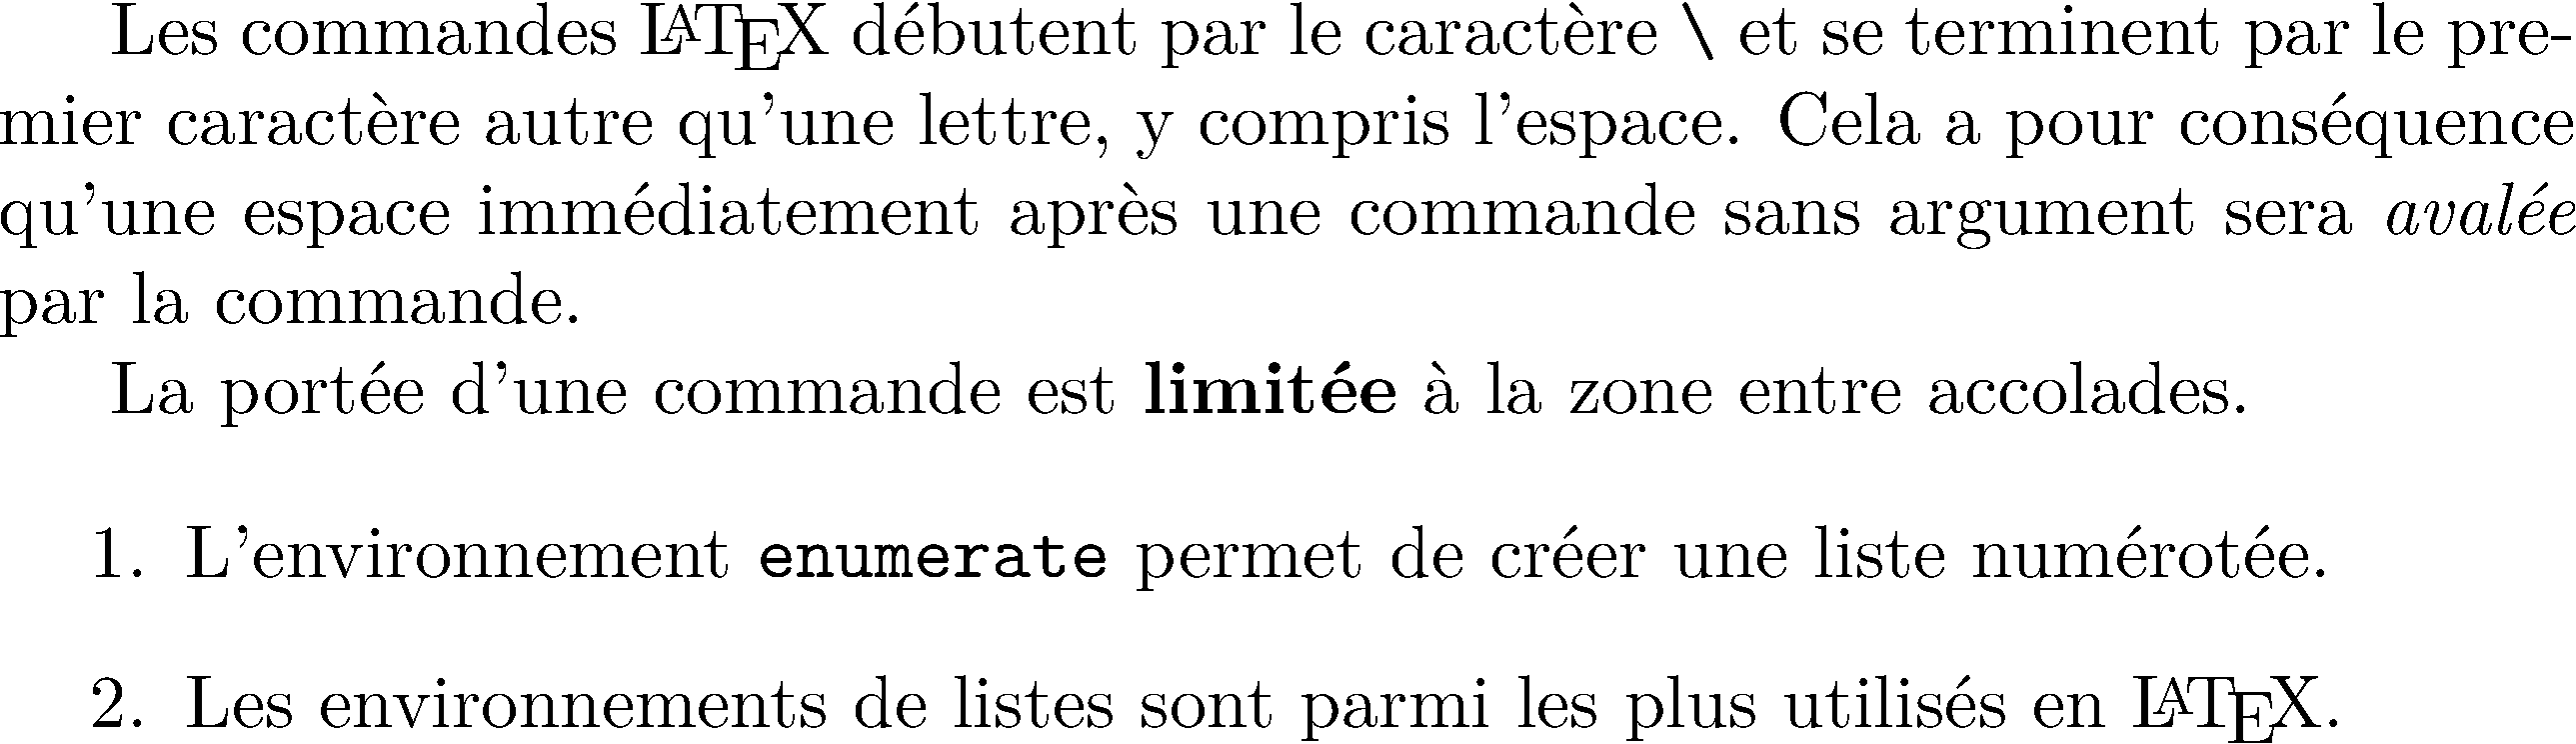
\includegraphics[width=0.95\linewidth]{exercice_commandes-output}
  \end{center}
\end{exercice}

\begin{exercice}[nosol]
  \begin{enumerate}
  \item Compiler tel que fourni le fichier
    \fichier{exercice\_classe+paquetages.tex}.
  \item Changer la police de caractère du document pour 11~points,
    puis 12~points. Changer la classe du document pour \class{memoir}.
    Observer l'effet sur les marges et sur la coupure automatique des
    mots.
  \item Charger le paquetage \pkg{icomma} et observer l'effet sur la
    formule mathématique.
  \item Charger le paquetage \pkg{numprint} avec l'option
    \verb=autolanguage= (\emph{après} le paquetage \pkg{babel}). Dans
    le code source de la formule mathématique, changer
\begin{lstlisting}
10 000
\end{lstlisting}
    pour
\begin{lstlisting}
\nombre{10000}
\end{lstlisting}
    et observer le résultat.
  \end{enumerate}
\end{exercice}


%%% Local Variables:
%%% mode: latex
%%% TeX-engine: xetex
%%% TeX-master: "formation-latex-ul"
%%% coding: utf-8
%%% End:
